Having tested all the classifiers and obtaining ther respected probabilities we proceed to try to improve the overall performance by combining each of the predictions of the classifiers.

A brief summary can be visualized in Table \ref{table:summaryLogLoss}
\begin{table}[h!]
	\centering
	\caption{Test scores per classifier}
	\begin{tabular}{| l | c | c |}
		\hline
		\textbf{Classifier} & \textbf{Train} & \textbf{Test}\\
		\hline
		KNearestClassifier & 8.104e-15 & 0.8702 \\ \hline
		LogisticRegression & 0.7078 & 0.7204 \\ \hline
		RandomForestClassifier & 0.1397 & 0.5497 \\ \hline
		GradientBoostingClassifier & 0.3610 & 0.4978 \\ \hline
	\end{tabular}
	\label{table:summaryLogLoss}
\end{table}

From here we proceed to:
\begin{itemize}
	\item Average all 4 predictions
	\item Obtain weights to minimize LogLoss
\end{itemize}

From averaging predictions the final LogLoss is:

$$ LogLoss_{mean} = 0.5204 $$

Weights found after minimizing the LogLoss can be visualized in Figure \ref{fig:weights}
\begin{figure}[h!]
	\centering
	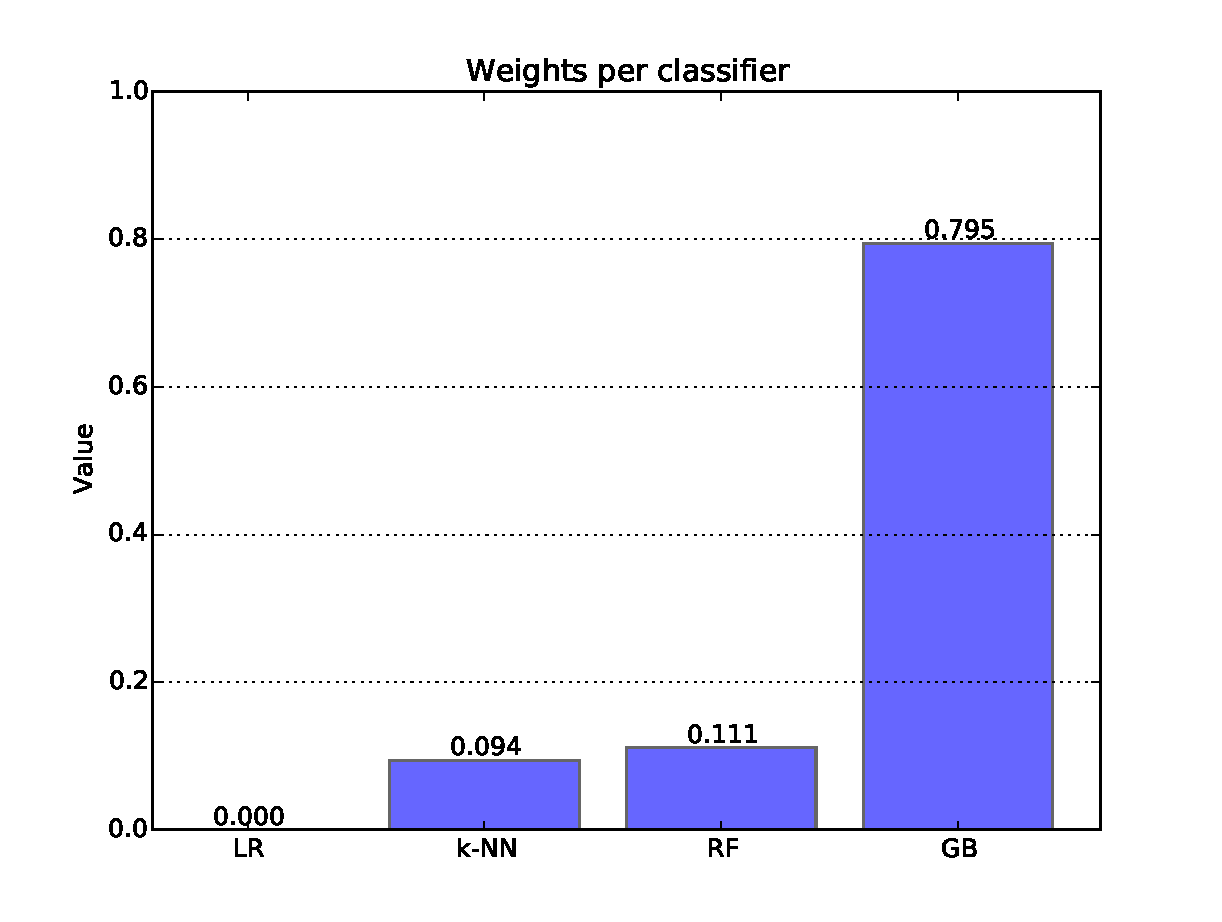
\includegraphics[width=0.8\textwidth]{weights}
	\caption{weights obtained from minimizing $LogLoss$ function}
	\label{fig:weights}
\end{figure}

$$ LogLoss_{weighted} = 0.4732 $$

The weights found can help ups identify which learning algorithms contribute the most to improving the LogLoss and which are practically useless. Indeed from Table \ref{table:summaryLogLoss} it can be foreseen that the output from Gradient Boosting would be one with most influence, however, even though the score using k-NN is the worst, it has nearly the same influence as Random Forest. Output obtained from Logistic Regression is practically useless given it's weight of $4.36e-7$.
